%\documentclass{sig-alternate-05-2015}
\documentclass{llncs}
\usepackage{makeidx}
\usepackage{tabularx,colortbl}
\usepackage[dvipsnames]{xcolor}
\usepackage{flushend}
\usepackage{cite}
\usepackage{amsmath}
%\usepackage{amsthm}
\usepackage{amssymb}
\usepackage{epsfig}
\usepackage{stmaryrd}
\usepackage{url}
\usepackage{multirow}
\usepackage{latexsym}
\usepackage{graphics}
\usepackage{graphicx}
\usepackage{enumitem}
\usepackage{comment}
\usepackage{longtable}
\usepackage{supertabular}
\usepackage{times}
\usepackage{listings}
\usepackage{subfigure}
\usepackage{color}
\usepackage{balance}
\usepackage{xspace}
\usepackage[ruled, vlined, linesnumbered]{algorithm2e}
\usepackage[autostyle]{csquotes}



%\theoremstyle{Definition}
%\newtheorem{definition}{Definition}
%%%
%\theoremstyle{Theorem}
%\newtheorem{theorem}{Theorem}


%\newcommand{\definition}{\noindent \textbf{Definition} \citation{}}
%\newcommand{\theorem}{\noindent \textbf{Theorem} \citation{}}
%\newcommand{\lemma}{\noindent \textbf{Lemma} \citation{}}

%\newdef{lemma}{Lemma}
%\newdef{definition}{Definition}
%\newdef{theorem}{Theorem}
%\newdef{corollary}{Corollary}
%\newdef{note}{Note}
%\newdef{axiom}{Axiom}
\newcommand{\mkeyword}[1]{\mbox{\texttt{#1}}}
\DeclareMathOperator{\kuop}{uop}
\DeclareMathOperator{\kbop}{bop}
\DeclareMathOperator{\kite}{ite}
\DeclareMathOperator{\kpre}{pre}
\DeclareMathOperator{\dom}{dom}
\DeclareMathOperator{\ktrue}{true}
\DeclareMathOperator{\kfalse}{false}
\DeclareMathOperator{\kselect}{select}
\DeclareMathOperator{\ran}{range}
\newcommand{\lbb}{[\![}
\newcommand{\rbb}{]\!]}
\newcommand{\expr}{\phi}
\newcommand{\exprS}{\Phi}
\newcommand{\mike}[1]{\textcolor{red}{#1}}
\newcommand{\mats}[1]{\textcolor{blue}{#1}}
\newcommand{\darren}[1]{\textcolor{green}{#1}}
\newcommand{\danielle}[1]{\textcolor{orange}{#1}}

\sloppypar



\begin{document}

\definecolor{gold}{rgb}{0.90,.66,0}
\definecolor{dgreen}{rgb}{0,0.6,0}
\newcommand{\stateequiv}{\equiv_{s}}
\newcommand{\traceequiv}{\equiv_{\sigma}}
\newcommand{\ta}{\text{TA}}
\newcommand{\cta}{\text{TA$_{C}$}}
\newcommand{\tta}{\text{TA$_{T}$}}
\newcommand{\ucalg}{\texttt{\small{IVC\_UC}}}
\newcommand{\ucbfalg}{\texttt{\small{IVC\_UCBF}}}


\title{Architectural Modeling and Analysis for Safety Engineering}
%
\author{Danielle Stewart\inst{1}
\and Michael W. Whalen\inst{1}
\and Darren Cofer\inst{2}
\and Mats P.E. Heimdahl\inst{1} }
\institute{University of Minnesota\\Department of Computer
Science and Engineering\\
200 Union Street\\
Minneapolis, MN, 55455, USA\\
\email{whalen, dkstewar, heimdahl@cs.umn.edu}
\and
Rockwell Collins\\
Advanced Technology Center\\400 Collins Rd. NE\\
Cedar Rapids, IA, 52498, USA\\ \email{ darren.cofer@rockwellcollins.com}
}
\maketitle

\begin{abstract}
Architecture description languages such as AADL allow systems engineers to specify the structure of system architectures and perform several analyses over them, including schedulability, resource analysis, and information flow.  In addition, they
permit system-level requirements to be specified and analyzed early in the development process of airborne and ground-based systems. These tools can also be used to perform safety analysis based on the system architecture and initial functional decomposition.

%Previously, Rockwell Collins and the University of Minnesota developed and demonstrated an approach to behavioral model-based safety analysis using Simulink. New MBSE tools that incorporate assume-guarantee compositional analysis techniques provide the basis for greatly improving earlier approaches to safety analysis and can be used to ensure model consistency, correctness of assumptions, and better scalability.

Using AADL-based system architecture modeling and analysis tools as an exemplar, we extend existing analysis methods to support system safety objectives of ARP4754A and ARP4761. This includes extensions to existing modeling languages to better describe failure conditions, interactions, and mitigations, and improvements to compositional reasoning approaches focused on the specific needs of system safety analysis. We develop example systems based on the Wheel Braking System in SAE AIR6110 to evaluate the effectiveness and practicality of our approach.
\end{abstract}

\keywords{Model-based systems engineering, fault analysis, safety engineering}

\section{Introduction}
\label{sec:intro}

Risk and safety analyses are important activities used to ensure that critical systems operate in an expected way. From nuclear power plants and airplanes to heart monitors and automobiles, critical systems are ubiquitous in our society. These systems are required to operate safely under nominal and faulty conditions. Guaranteeing that system safety properties hold in the presence of faults is an important aspect of critical systems development and falls under the discipline of safety analysis. Safety analysis produces various safety related artifacts that are used during development and certification of critical systems~\cite{SAE:ARP4761,SAE:ARP4754A}. Examples include {\em minimal cut sets} -- the minimal sets of faults that may violate a safety property and {\em fault trees} -- the Boolean formula whose literals are minimal cut sets. Since the introduction of minimal cut sets in the field of safety analysis~\cite{vesely1981fault}, much research has been performed to address the generation of these sets and associated formulae~\cite{fta:survey,rauzy1993new,historyFTA,Bozzano:2010:DSA:1951720,rausand2003system}. As critical systems get larger, more minimal cut sets are possible with increasing cardinality. In recent years, symbolic model checking has been used to address scaling the analysis of systems with millions of minimal cut sets~\cite{bieber2002combination,schafer2003combining,fta:survey,contractBasedDesign,symbFTA,DBLP:conf/cav/BozzanoCPJKPRT15}. 

The state space explosion problem often prevents formal verification from being used on large systems. This problem can arise from combining parallel processes together and attempting to reason monolithically over them. Compositional reasoning takes advantage of the hierarchical organizaton of a system model. A compositional approach verifies each component of the system in isolation and allows global properties to be inferred about the entire system~\cite{berezin1997compositional}. The {\em assume-guarantee} paradigm is commonly used in compositional reasoning where the assumed behavior of the environment implies the guaranteed behavior of the component ~\cite{NFM2012:CoGaMiWhLaLu}.

Using an assume-guarantee reasoning framework, we extend the definition of the nomimal transition system to allow for unconstrained guarantees. We use this idea to generate all counterexamples to a proof for each layer of analysis, and then transform the results into a Boolean formula describing the satisfiability of the violation of a property. These results are then composed. 

After we provide the formalization, we describe the implementation in the OSATE tool for the Architecture and Analysis Lanugage (AADL)~\cite{FeilerModelBasedEngineering2012}. AADL has two annexes that are of interest to us: the Assume-Guarantee Reasoning Environment (AGREE)~\cite{NFM2012:CoGaMiWhLaLu} and the safety annex~\cite{stewart2020safety}. AGREE provides the assume-guarantee reasoning required for the transition system extension and the safety annex allows us to define faults on component outputs. 

Recently, Ghassabani et al. developed an algorithm that traces a safety property to a minimal set of model elements necessary for proof; this is called the \textit{all minimal inductive validity core} algorithm (\aivcalg)~\cite{GhassabaniGW16,Ghassabani2017EfficientGO,bendik2018online}. Inductive validity cores produce the minimal set of model elements necessary to prove a property. Each set contains the \emph{behavioral contracts} -- the requirement specifications for components -- used in a proof. We collect all MIVCs per layer to generate the minimal cut sets and thus the fault trees to be composed.

%The \aivcalg algorithm gives the minimal set of contracts required for proof of a safety property. If all of these sets are obtained, we have insight into every proof path for the property. Thus, if we violate at least one contract from every MIVC set, we have in essence ``broken" every proof path. This is the information that is used to perform fault analysis using MIVCs.

%If all of these sets are obtained, we have insight into not only what is necessary for the verification of the property, but we can also find what combination of contracts, if \emph{violated}, will provide a state of the system which makes the safety property unprovable. 

%Safety analysts are often concerned with faults in the system, i.e., when components or subsystems deviate from nominal behavior, and the propagation of errors through the system. To this end, the model elements included in the reasoning process of the \aivcalg algorithm are not only the contracts of the system, but faults as well. This will provide additional insight into how an active fault may violate contracts that directly support the proof of a safety property. 

%In complex critical systems, safety analysts are concerned with hardware faults, how these may propagate to software components reliant on the failed hardware, and other faults whose propagation requires insight into system dynamics. Scaling model checking of complex hardware and software is challenging;  one way to address this problem is to take advantage of the architecture of the system model through a \textit{compositional} approach~\cite{anderson1996model, clarke1989compositional,mcmillan1999verification}. Compositional model checking reduces the verification of a large system into multiple smaller verification problems that can be solved independently and which together guarantee correctness of the original problem.  One way to structure compositional verification is hierarchically: layers of the system architecture are analyzed independently and their composition demonstrates a system property of interest.

This paper presents a compositional approach to generating fault forests (finite sequences of fault trees) and minimal cut sets, allowing us to reason uniformly about faults in hardware and software and their impact (propagation) to system properties. The main contributions of this research include the formalization of the composition of fault forests and its implementation.


The organization of the paper is as follows.  Section 2 describes a running example, Section 3 outlines the formalization of this approach. The implementation of the algorithms is discussed in Section 4 and 5 and related work follows in Section 6. The paper ends with a conclusion and discussion of future work.


%\section{Safety Assessment Process}
\label{sec:process}
%\mike{COMPLETELY STOLEN FROM THE SAFECOMP-05 PAPER!  Either note it or modify it}
%\danielle{I added a citation. I think this late in the game we might as well just cite it.}

The overall safety assessment process that is followed in practice
in the avionics industry is described in the SAE standard ARP
4761~\cite{SAE:ARP4761}. This section is a summarization of portions of the ARP 47-61 document (also found in~\cite{Joshi05:SafeComp}). 

\iffalse

This section describes the overall safety assessment process that is followed in
practice in the avionics industry along the lines of the SAE standard ARP 47-61 \cite{SAE:ARP4761}. The descriptions of the various phases of the safety assessment process
covered in this section are essentially based on the ARP 47-61 document.

\fi


\begin{figure}
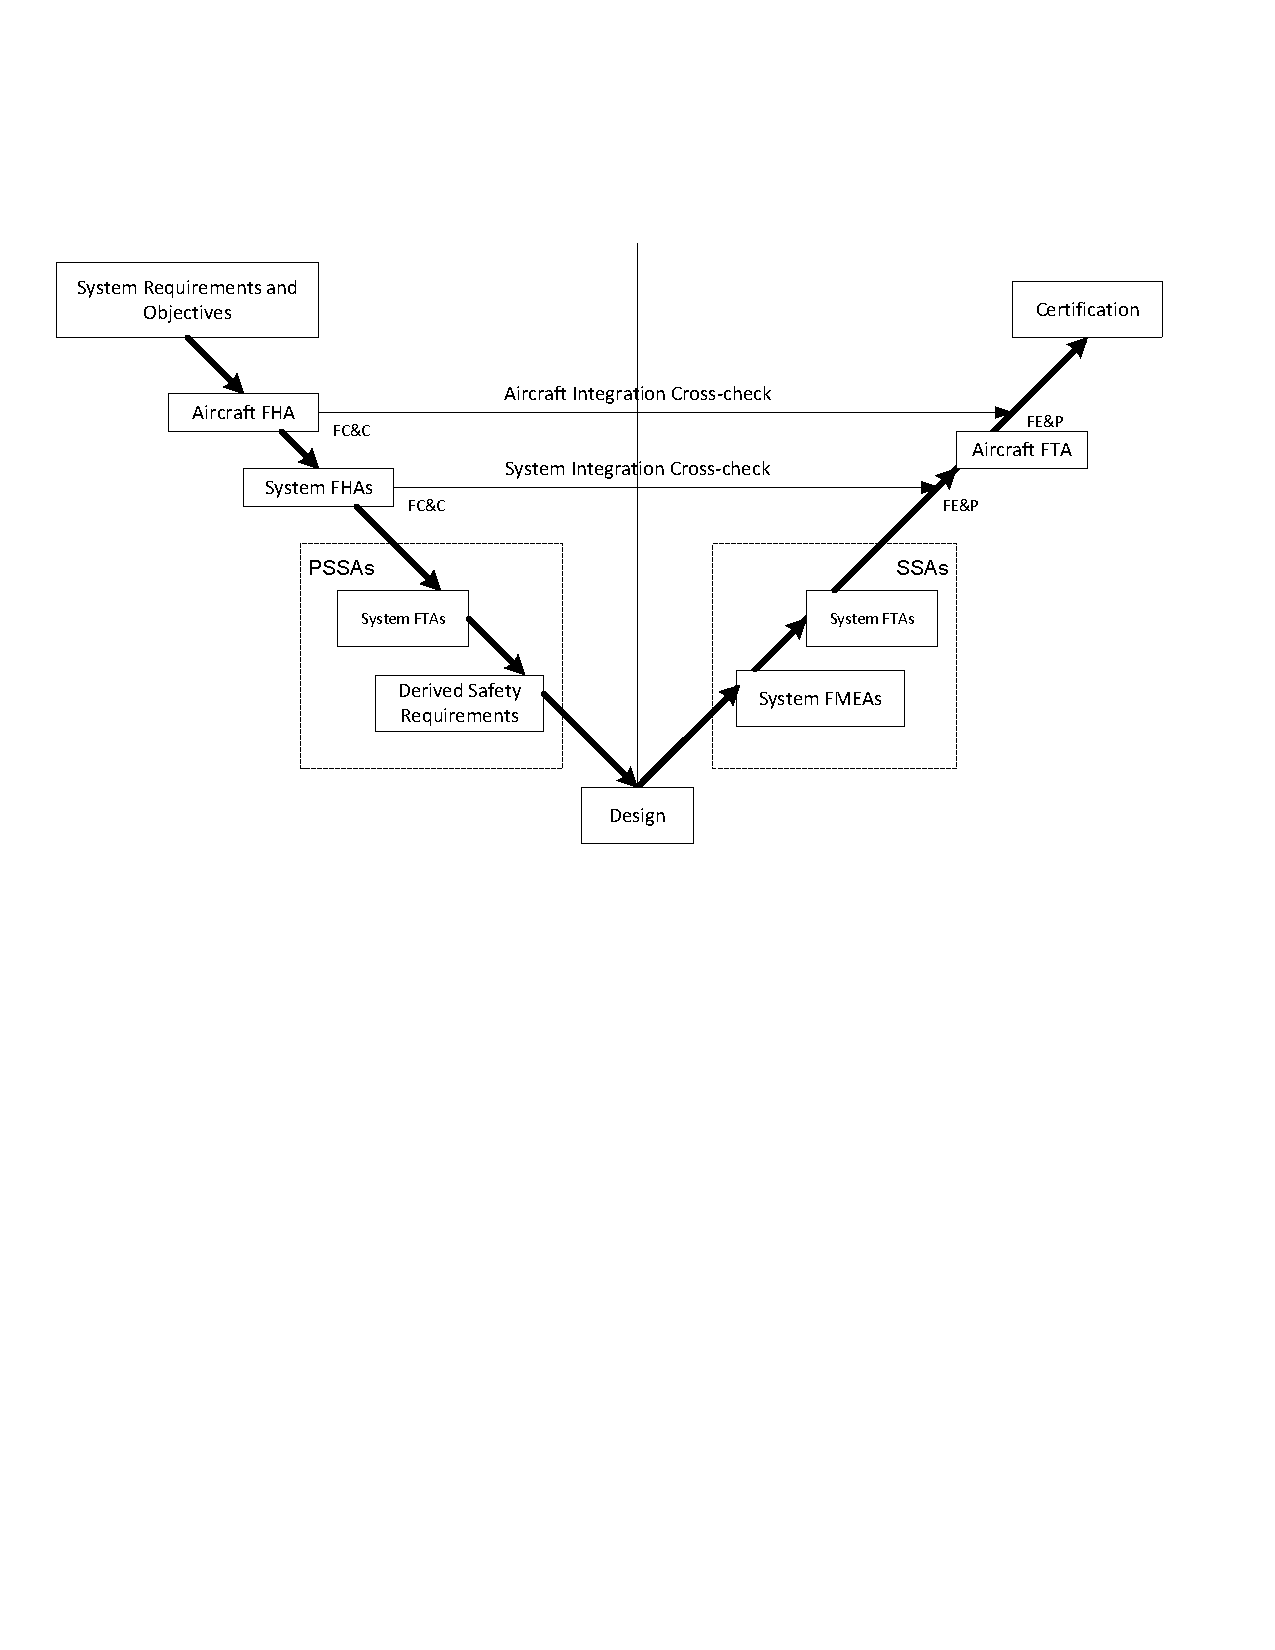
\includegraphics[trim=25 375 0 125, clip, scale=.60]{V}
\caption{Traditional ``V'' Safety Assessment Process} \label{fig:V}
\end{figure}

%The safety assessment process is an integral part of the development process.

Figure~\ref{fig:V} shows an overview of the safety assessment
process as recommended in ARP 4761. The process includes safety
requirements identification (the left side of the ``V'' diagram)
and verification (the right side of the ``V'' diagram), that
support the aircraft development activities. An aircraft level
Functional Hazard Analysis (FHA) is conducted at the beginning of
the aircraft development cycle, which is then followed by system
level FHA for individual sub-systems. The FHA is followed by
Preliminary System Safety Assessment (PSSA), which derives safety
requirements for the subsystems, primarily using Fault Tree
Analysis (FTA). The PSSA process iterates with the design
evolution, with design changes necessitating changes to the
derived system requirements (and also to the fault trees) and
potential safety problems identified through the PSSA leading to
design changes. Once design and implementation are completed, the
System Safety Assessment (SSA) process verifies whether the safety
requirements are met in the implemented design. The system Failure
Modes and Effects Analysis (FMEA) is performed to compute the
actual failure probabilities on the items. The verification is
then completed through quantitative and qualitative analysis of
the fault trees created for the implemented design, first for the
subsystems and then for the integrated aircraft.

%\medskip

We propose to modify this traditional ``V'' process so that the
lower level PSSA and SSA activities are performed based on a
formal model of the system under consideration.
Figure~\ref{fig:Vmod} shows the modified ``V'' diagram for
model-based safety analysis. The shaded blocks are those
activities that will be modified or added.

\begin{figure}
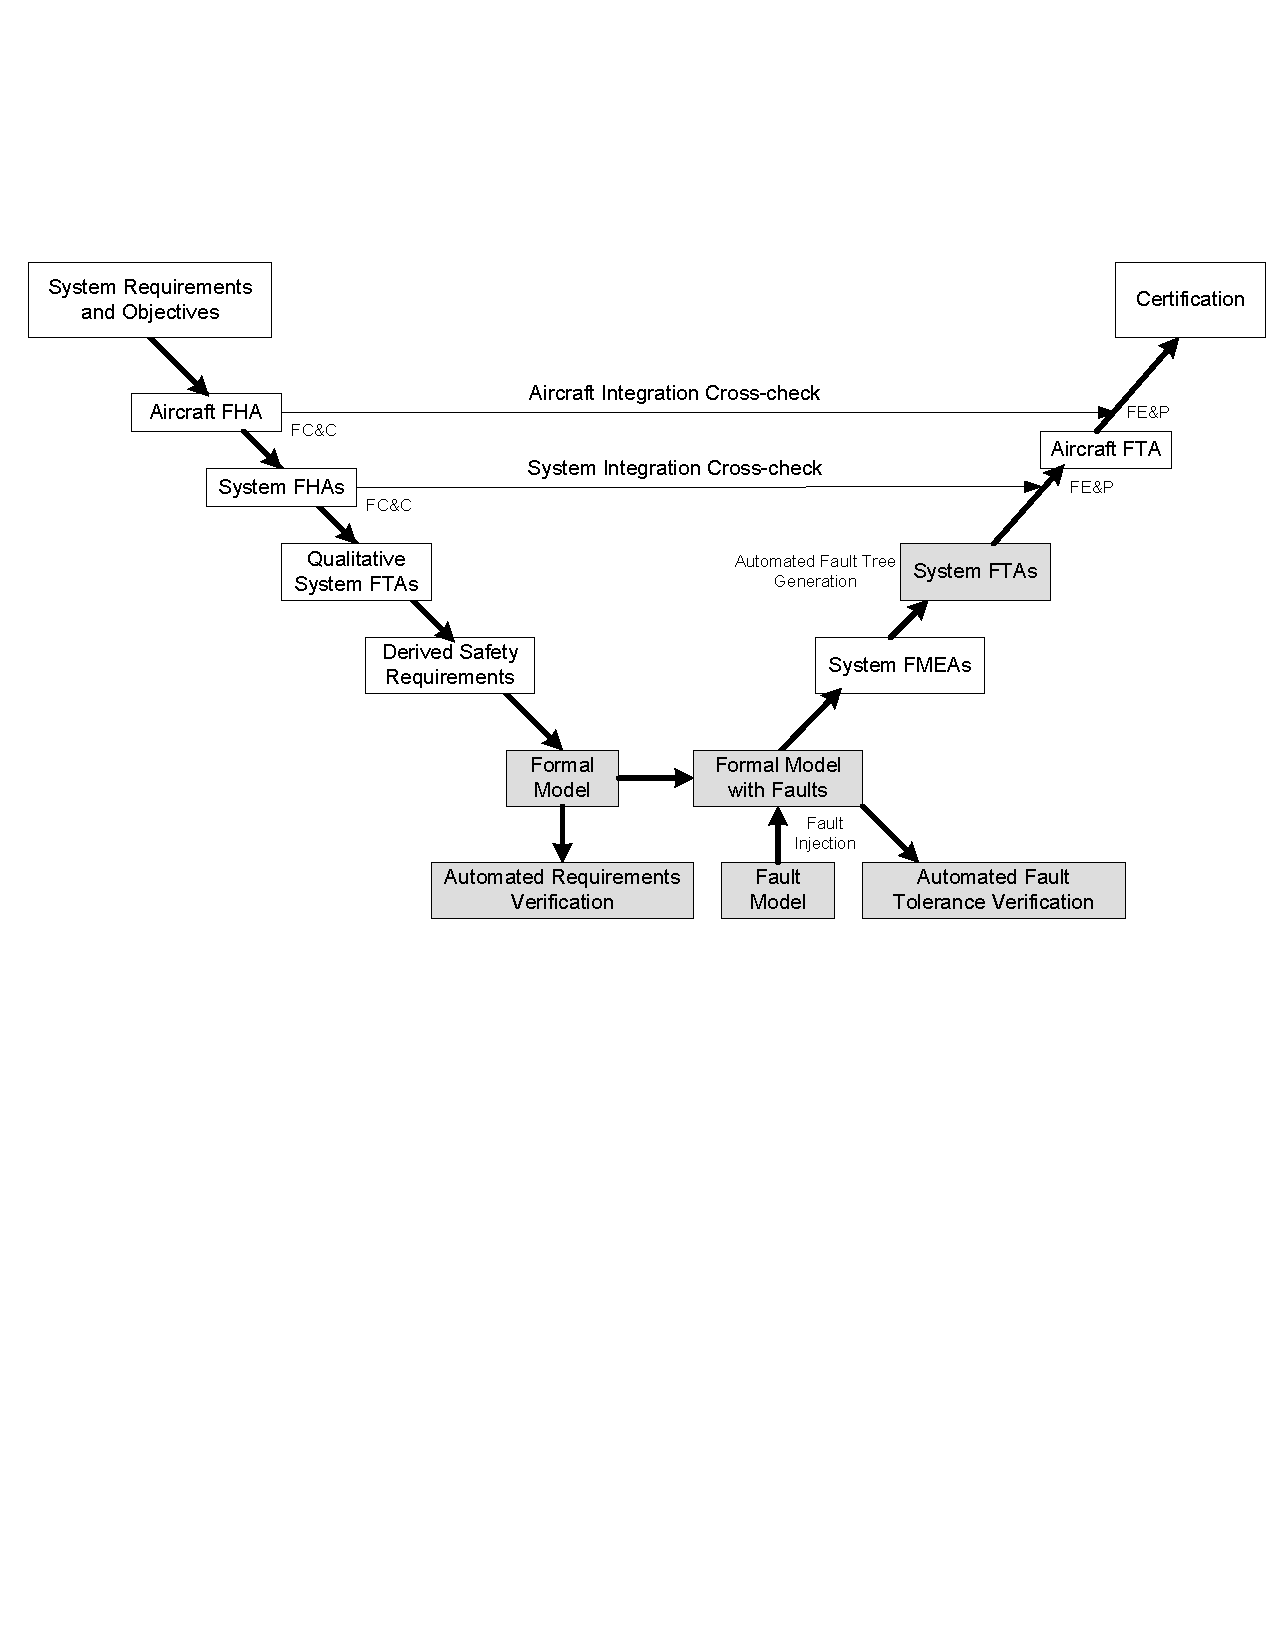
\includegraphics[trim=15 350 0 125, clip, scale=.60]{Mod_V_Process_FaultModel}
\caption{Modified ``V'' Safety Assessment Process} \label{fig:Vmod}
\end{figure}


As we can observe from Figure~\ref{fig:Vmod}, the parts of the analysis that are
primarily affected are at the bottom of the ``V''. The biggest difference is that
the safety analysis activities at this level are now focused around a formal
model of the system behavior, and that many of the artifacts of the safety
analysis can be derived from this model. The idea is to try to pose the right
verification questions to formal tools (such as model checkers and theorem
provers) so that it is possible to derive the necessary safety analysis
information. We then wish to turn the results of these analyses back into
artifacts that can be easily understood and used by safety engineers.


\section{Example: Wheel Brake System}

%\mike{Move the generic description to a section right after the ``safety'' section along with the ARP figure.  Leave the modeling that we did in AADL here.  That way we can reference it in the MBSA sections.}
%\danielle{The whole nominal model description is here. The modeling we did is in the faults section.}

As a preliminary case study, we utilized the Wheel Brake System (WBS) described in \cite{AIR6110} (previously found in ARP4761 Appendix L). This ficticious aircraft system was developed to illustrate the design and safety analysis principles of ARP4754A and ARP4761.  The WBS is installed on the two main aircraft landing gears and is used during taxi, landing, and rejected take off. Braking is either commanded manually using brake pedals or automatically by a digital control system with no need for the pedals (autobrake). When the wheels have traction, the autobrake function will provide a constant smooth deceleration.

\begin{figure}
\begin{center}
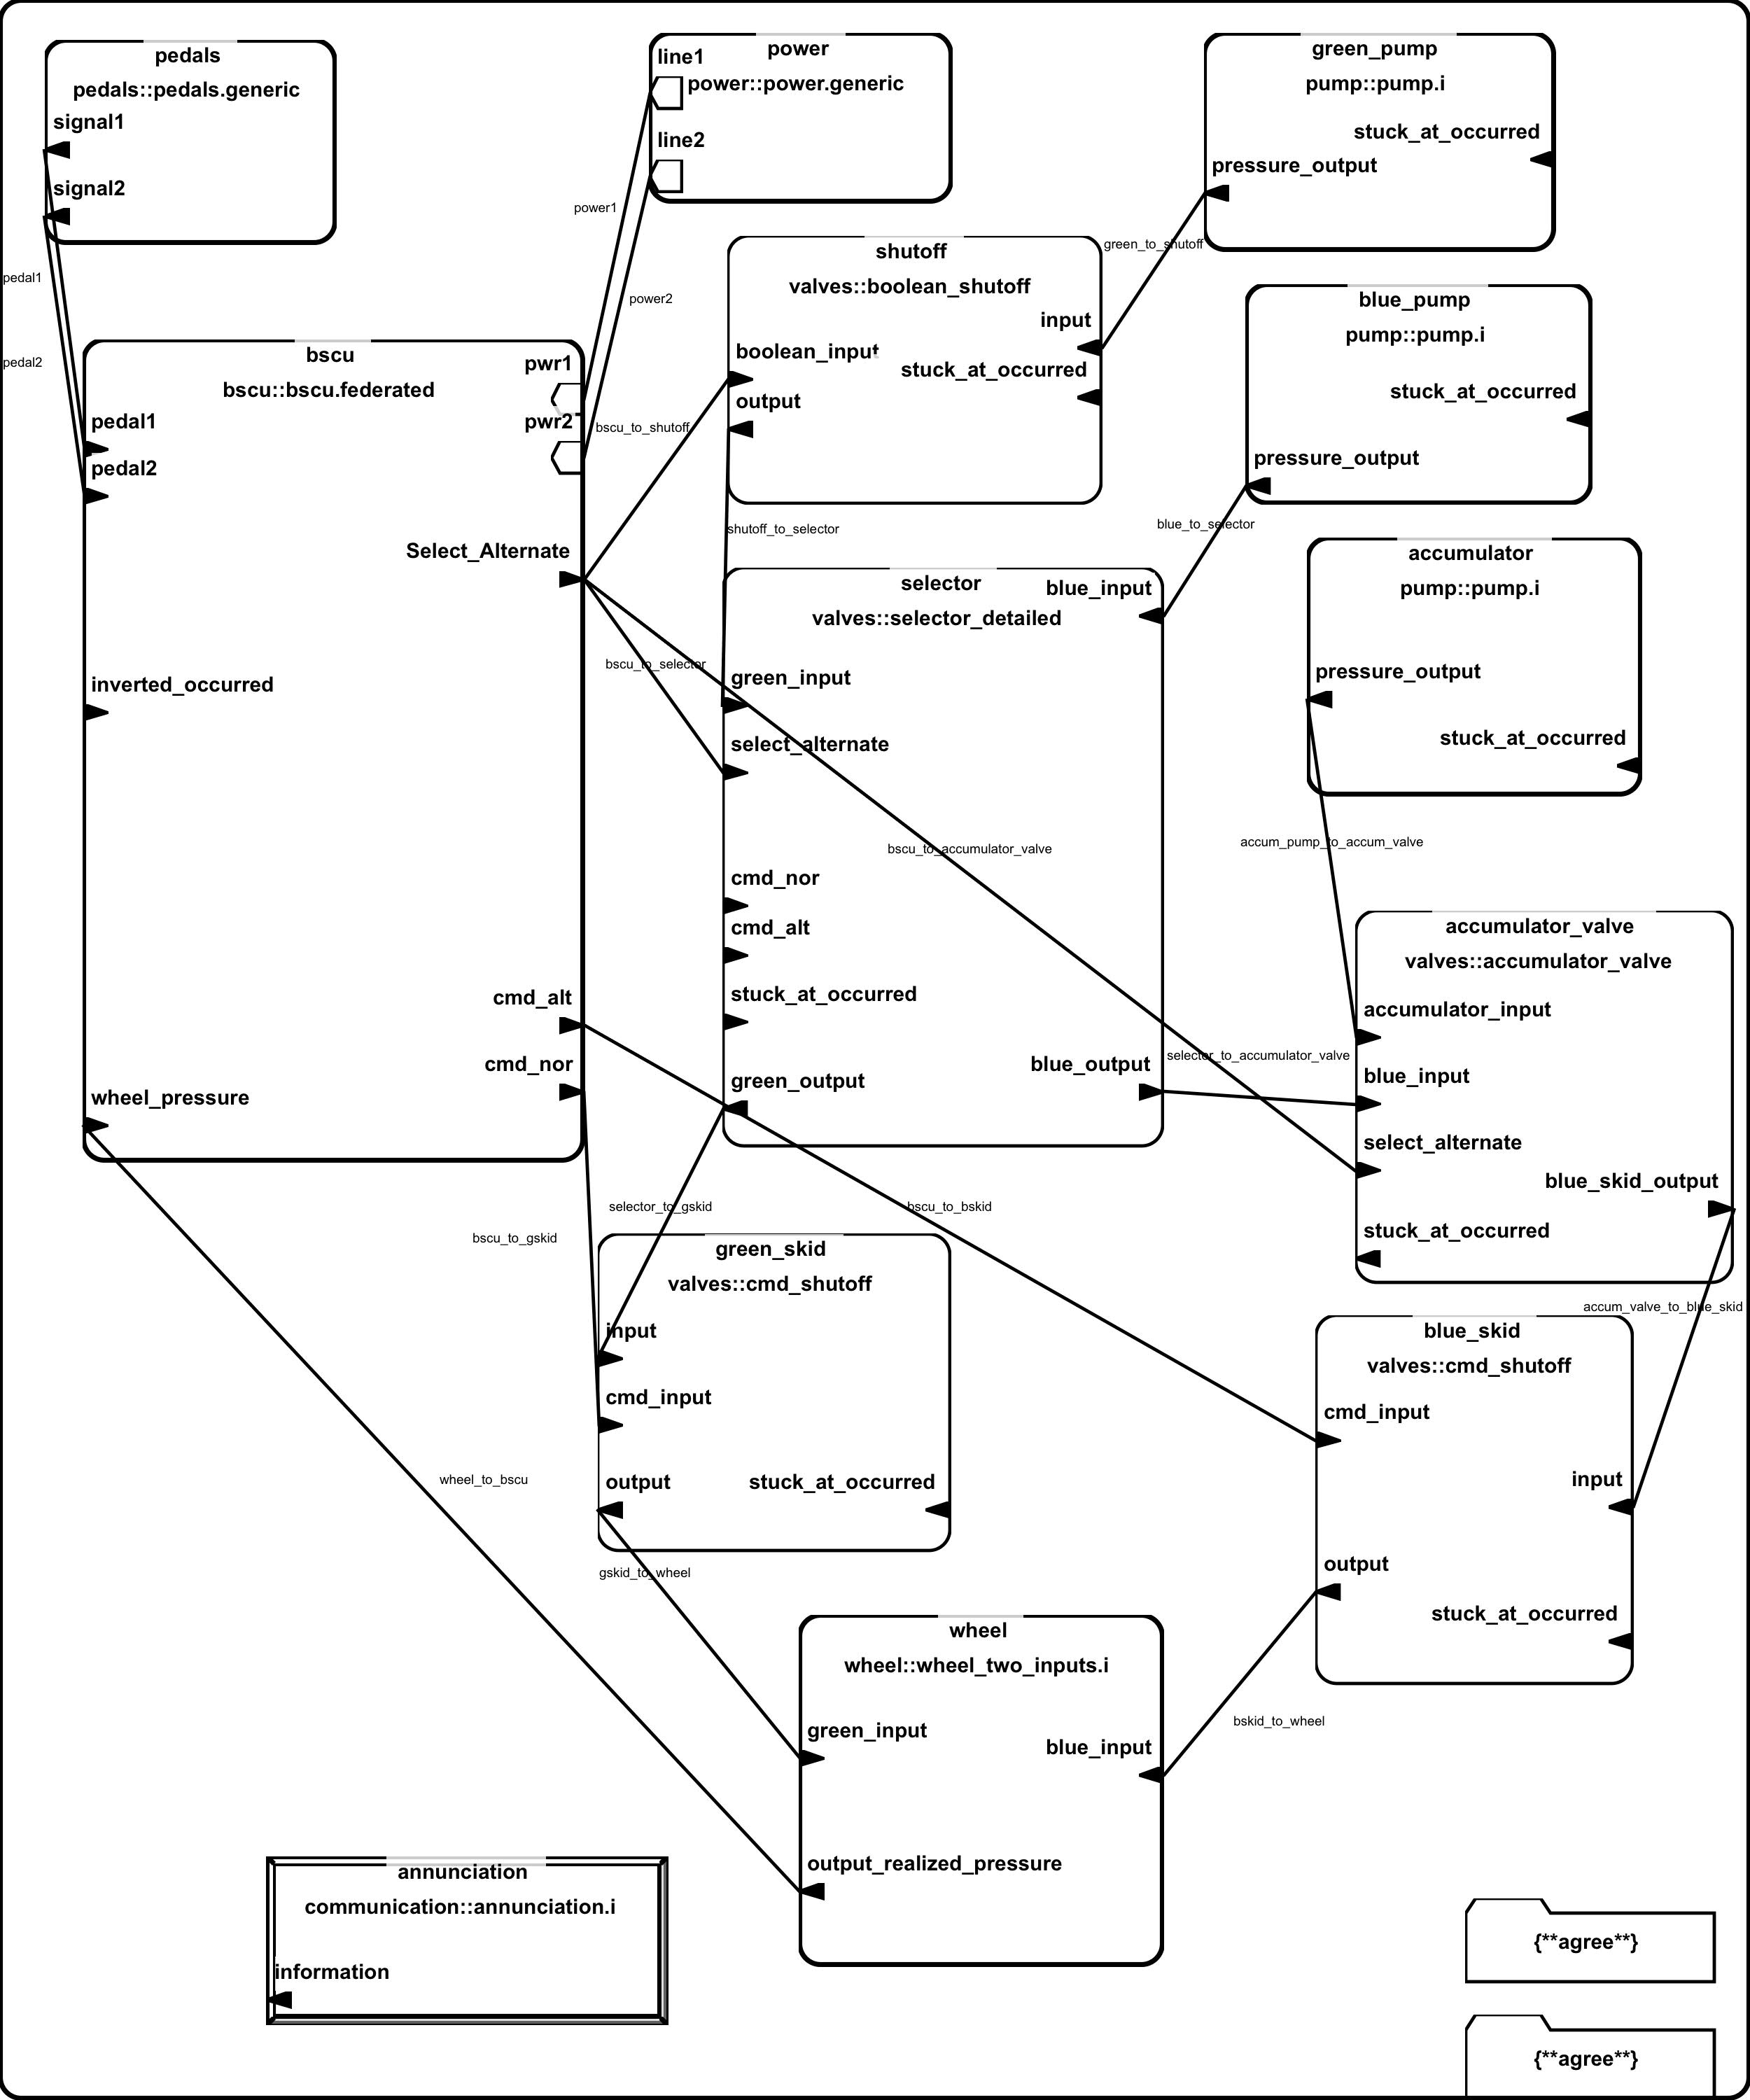
\includegraphics[width=\textwidth]{images/wbsfederated3.jpg}
\caption{AADL Simple Model of the Wheel Brake System }
\label{fig:wbs_ima}
\end{center}
\end{figure}

Each wheel has a brake assembly that can be operated by two independent hydraulic systems (designated green and blue). In normal braking mode, the green hydraulic system operates the brake assembly.  If there is a failure in the green hydraulics, the system switches to alternate mode which uses the blue hydraulic system.  The blue system is also supplied by an accumulator which is a device that stores hydraulic pressure that can be released if both of the primary hydraulic pumps (blue and green) fail. The accumulator supplies hydraulic pressure in Emergency braking mode.

Switching between the hydraulic pistons and pressure sources can be commanded automatically or manually. If the hydraulic pressure in the green supply is below a certain threshold, there is an automatic switchover to the blue hydraulic supply. If the blue hydraulic pump fails, then the accumulator is used to supply hydraulic pressure.

In both normal and alternate modes, an anti-skid capability is available. In the normal mode, the brake pedal position is electronically fed to a computer called the Braking System Control Unit (BSCU). The BSCU monitors signals that denote critical aircraft and system states to provide correct braking function, detect anomalies, broadcast warnings, and sent maintenance information to other systems.

\subsection{Nominal System Model}
\label{sec:nominal}
The WBS AADL model of the nominal system behavior consists of mechanical and digital components and their interconnections, as shown in Figure~\ref{fig:wbs_ima}. The following section describes this nominal model from which the fault model was generated.

\paragraph{Wheel Braking System (WBS)}
The highest level model component is the WBS. It consists of the BSCU, green and blue hydraulic pressure lines (supplied by the green pump  and blue pump/accumulator respectively), a Selector which selects between normal and alternate modes of hydraulic pressure, and the wheel system. The WBS takes inputs from the environment including PedalPos1, AutoBrake, DecRate, AC\_Speed, and Skid. All of these inputs are forwarded to the BSCU to compute the brake commands.

\paragraph{Braking System Control Unit (BSCU)}
The BSCU is the digital component in the system that receives inputs from the WBS. It also receives feedback from the green and blue hydraulic lines and two power inputs from two separate power sources. The BSCU is composed of two command and monitor subsystems each powered independently from separate power sources. The pedal position is provided to these units and when skidding occurs, the command and monitor units will decrease the pressure to the brakes.
The command unit regulates the pressure to the brakes in the green hydraulic line through the command cmd\_nor. Computing this command requires both the brake requested power and the skid information. The command unit also regulates the pressure in the blue hydraulic line in order to prevent skidding which it does through the cmd\_alt command. The monitor unit checks the validity of the command unit output.

The BSCU switches from normal to alternate mode (blue hydraulic system) when the output from either one of its command units is not valid or the green hydraulic pump is below its pressure threshold.  Once the system has switched into alternate mode, it will not switch back into normal mode again.

\paragraph{Hydraulic Pumps}
There are three hydraulic pumps in the system, green pump (normal mode), blue pump (alternate mode), and accumulator pump (emergency mode). Each pump provides pressure to the system and is modeled in AADL as a floating point value.

\paragraph{Shutoff Valve}

The shutoff valve is situated between the green pump and the selector. It receives an input from the BSCU regarding valve position and regulates the pressure coming through the green pipe accordingly.

\paragraph{Selector Valve}
The selector receives inputs from the pumps regarding pressure output and the BSCU regarding which mode the system is in. It will output the appropriate pressure from green, blue, or accumulator pump. An added requirement of the selector system is that it will only output pressure from one of these sources. Thus, the case of having pressure supplied to the wheels from more than one pump is avoided. The Selector takes the two pipe pressures (green and blue) as input, selects the system with adequate pressure and blocks the system with inadequate pressure. If both systems have pressure greater than the threshold, the AADL selects normal mode as the default.

\paragraph{Skid Valves}
The blue\_skid and green\_skid valves receive input from the selector as pressure coming through the respective pipes as well as input from the BSCU that commands normal or alternate mode. The skid valves will use these inputs to choose between the green or the blue pressure to send to the wheel.

\subsection{Modeling Nominal System Behavior}
In order to reason about behaviors of complex system architectures, we have developed a compositional verification tool for AADL models.
Our tool, the {\em Assume-Guarantee Reasoning Environment} (AGREE) \cite{NFM2012:CoGaMiWhLaLu}  is based on {\em assume-guarantee} contracts that can be added to AADL components.  The language used for contract specification is based on the LUSTRE dataflow language~\cite{Halbwachs91:IEEE}. The tool allows scaling of formal verification to large systems by splitting the analysis of a complex system architecture into a collection of verification tasks that correspond to the structure of the architecture.

We use AGREE to specify behavioral contracts corresponding to the behaviors expected of each of the WBS components. An example of a contract is shown in Figure~\ref{fig:agreeContract}.
%

\begin{figure}
\begin{center}
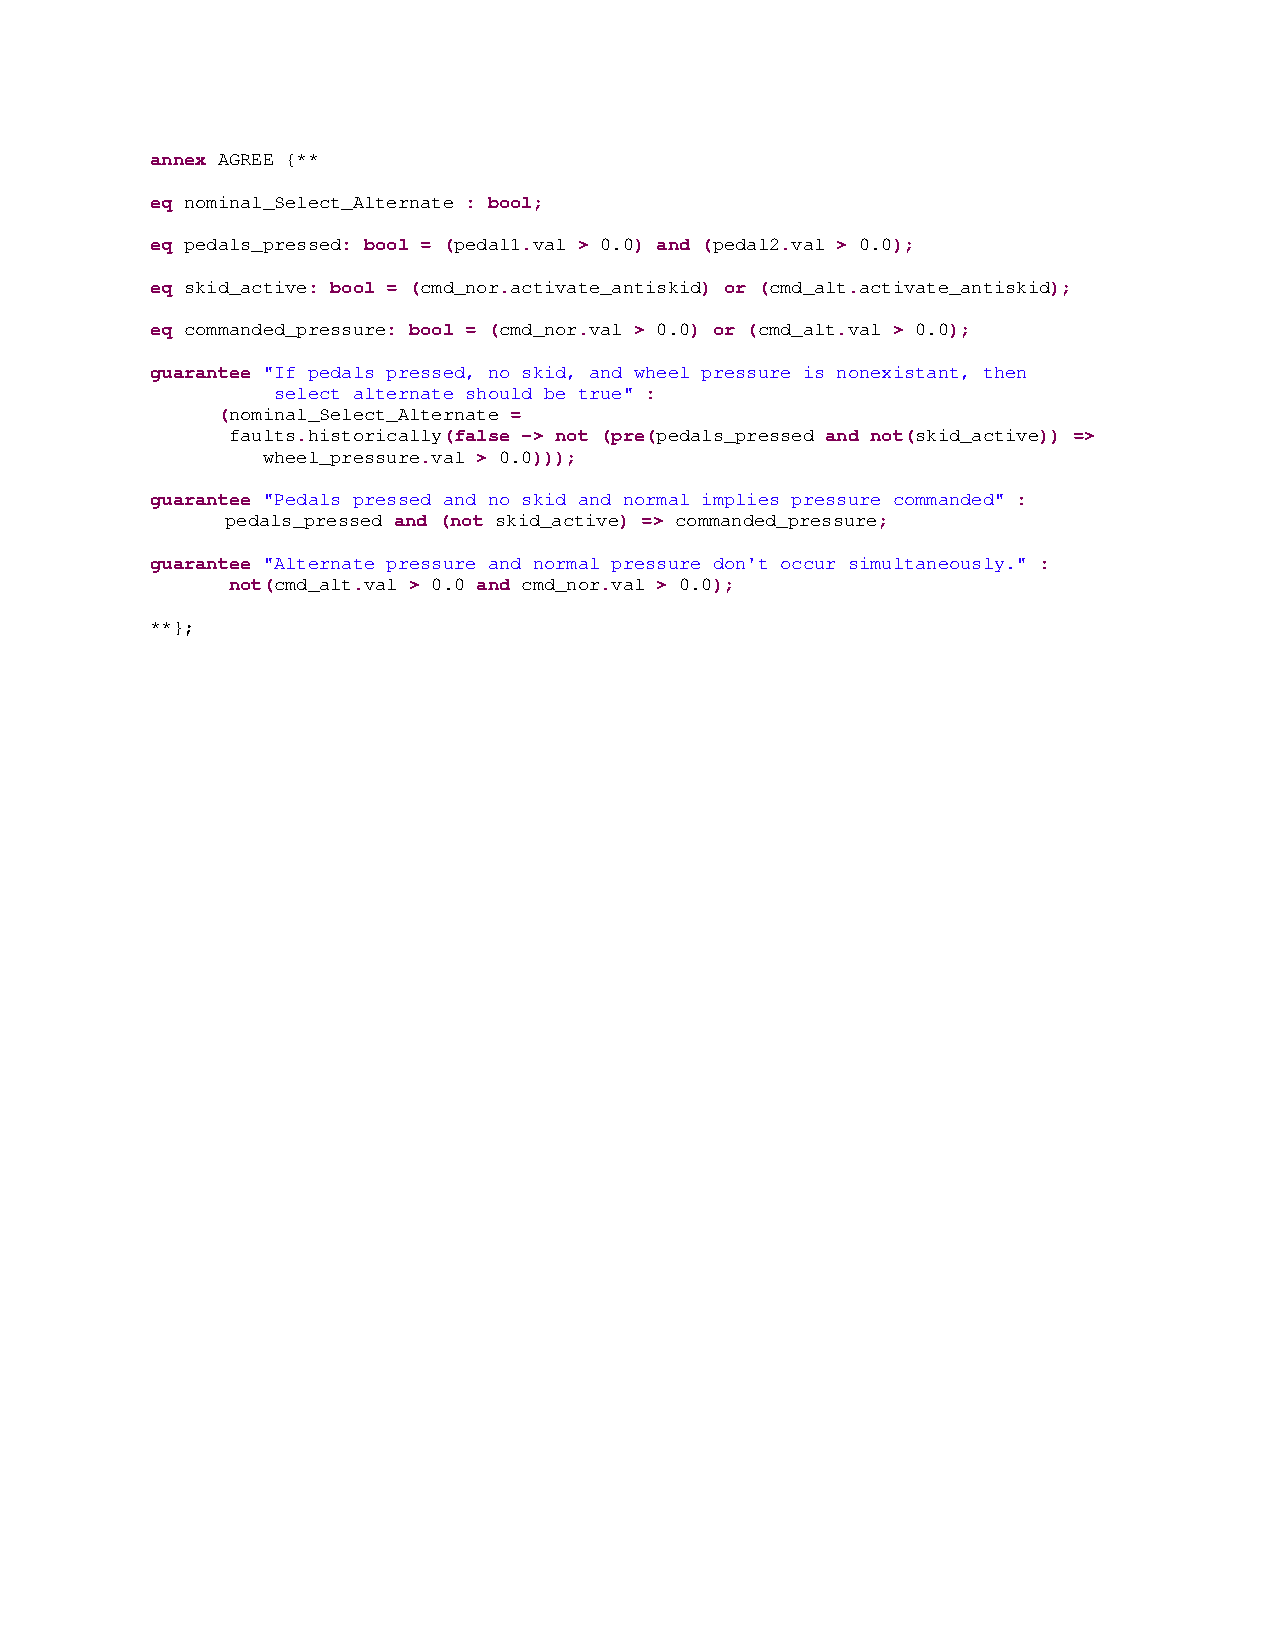
\includegraphics[trim=60 480 50 60,clip,width=\textwidth]{images/bscu.pdf}
\caption{AGREE Contract for BSCU }
\label{fig:agreeContract}
\end{center}
\end{figure}

\iffalse

\subsection{Nominal System Modeling}
\mike{KEEP HERE!}
A formal specification of the nominal system model consists of mechanical and digital components and their interconnections.

The highest level component is the Wheel Braking System (WBS). It consists of a digital control unit, the BSCU, and normal and alternate hydraulic pressure lines (supplied by green pump and blue pump/accumulator respectively). The system takes inputs from the environment including PedalPos1, AutoBrake, DecRate, AC\_Speed, and Skid. All of these inputs are forwarded to the BSCU to compute the brake commands. The outputs of the WBS are normal\_pressure, alternate\_pressure, and System\_Mode (normal, alternate, EMERGENCY).

\subsection{Braking System Control Unit (BSCU)}
The BSCU is the digital component in the system that receives inputs from the WBS. It also receives feedback from the normal and alternate lines and two power inputs from two separate power sources.

\fi



\section{Preliminaries}
\label{sec:background}
One of our goals is to transition the tools we have developed into use by the safety engineers who perform safety assessment of avionics products. Therefore, we need to understand how the tools and the models will fit into the existing safety assessment and certification process. Part of this understanding involves taking a look at pertinent background information in safety analysis. 

\subsection{Safety Critical Systems}
\label{sec:SA_background}
A safety critical system is a system whose safety cannot be shown solely by test, whose logic is difficult to comprehend without the aid of analytical tools, and whose failure can directly or indirectly cause significant loss of life or property\cite{SAE:ARP4761}. Guaranteeing safety and reliability of safety critical systems is mandatory. The process that guides this guarantee is highly standardized and controlled~\cite{RTCA:StdC,SAE:ARP4761} . Due to the complexity of critical systems, the field of safety analysis has in recent decades turned to formal methods~\cite{mattarei,Bozzano:2010:DSA:1951720}. In practice, a systems behavior can be described in a variety of ways that include diagrams, textual descriptions, and operational procedures~\cite{SAE:ARP4754A}. These descriptions must be clear and well defined in order to avoid ambiguous interpretation. The formal definition of system behavior has a unique interpretation and is therefore a good candidate for automated analysis in order to validate requirements and spot design flaws~\cite{Joshi05:Dasc}. 

Model checking is a technique used to allow exhaustive and automatic checking of whether a system model (formal system definition) meets a set of formal requirements. As early as the '90's, using model checking for safety requirements began to surface in the critical systems literature\cite{DBLP:conf/safecomp/CimattiGMRTT98,DBLP:conf/edcc/BernardeschiFGM96}. Current tools in safety analysis use model checking techniques during the development and assessment of safety critical systems, \cite{mattarei,CAV2015:BoCiGrMa,symbAltaRica,DBLP:conf/tacas/BittnerBCCGGMMZ16}.







\subsection{Model Based Safety Analysis}
\label{sec:mbsa}

Safety engineers traditionally perform safety analysis based on information synthesized from a variety of sources including informal design models and requirement documents. These analyses are highly subjective and dependent on the skill of the analyst. The lack of precise models requires the analyst to devote a fair amount of time to information gathering of the architecture and behavior of the system. On the other hand, in Model Based Safety Aanalysis (MBSA), the system and safety engineers share a common system model created using the model based development process. By extending the system model and relevant physical control systems, automated support can be provided for much of the safety analysis. Using a common model for both system and safety engineering and automating parts of safety analysis assists in the reduction of cost and improves the quality of the safety analysis, but this is not without disadvantages if the model itself is faulty. 

In model based system development, various development activities such as simulation, verification, testing, and code generation are based on a formal model of the system under development\cite{Joshi05:Dasc}. This is called the nominal model. Model based development was extended to include model based safety analysis\cite{Joshi05:Dasc,Joshi05:SafeComp,Joshi07:Hase,DBLP:conf/cav/BozzanoCPJKPRT15,CAV2015:BoCiGrMa,info17:HaLuHo}. The goal of MBSA is to incorporate safety analysis into the model based development process in order to provide information on the safety of the formal model of the system under development. In this process, the nominal (non-failure) system behavior that is captured in the model based development process is augmented with the fault behavior of the system. Model based safety analysis then operates on a formal model that describes both nominal system behavior and the fault model, which describes fault behavior. 






\subsection{Safety Assessment Process}
\label{subsec:process}

ARP4761, the Guidelines and Methods for Conducting Safety Assessment Process on Civil Airborne Systems and Equipment, provides guidance on applying development assurance at each hierarchical level throughout the development life cycle of highly-integrated/complex aircraft systems, and has been recognized by the Federal Aviation Administration (FAA) as an acceptable method to establish the assurance process~\cite{SAE:ARP4761}.

\begin{figure*}[h!]
	%\vspace{-0.956in}
	\centering
	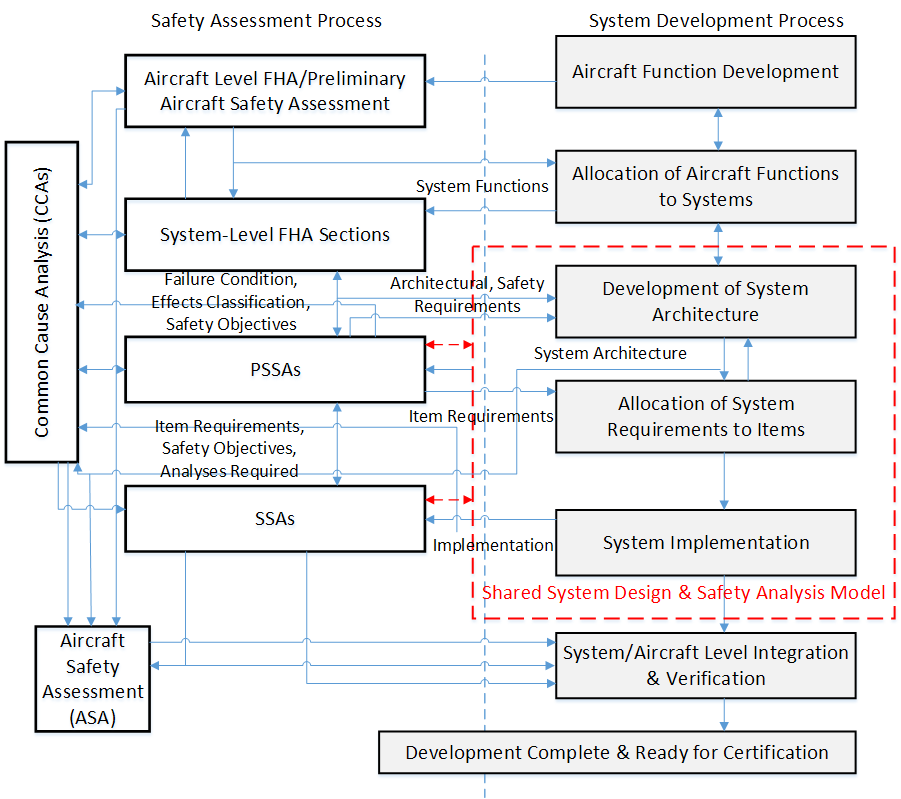
\includegraphics[width=1.0\textwidth]{images/Safety_Assessment_Process.png}
	%\vspace{-0.4in}
	\caption{Using the Shared System/Safety Model in the ARP4754A Safety Assessment Process}
	\label{fig:proposed_safety_process}
\end{figure*}

The safety assessment process is part of the development life cycle, and is tightly coupled with the system development and verification processes. It is used to show compliance with certification requirements and for meeting a company's internal safety standards. The guidelines presented in ARP4761 include various industry accepted safety assessment practices. They are summarized here for convenience. 

\begin{itemize}
\item Functional Hazard Assessment (FHA): This process examines aircraft and system functions to identify potential functional failures and classifies the hazards associated with specific failure conditions. This is usually developed early in the development process and is updated throughout. 

\item Preliminary System Safety Assessment (PSSA): This will establish the system safety requirements and provide some indication that the system architecture can meet those safety requirements. This is also updated throughout the development process.

\item System Safety Assessment (SSA): This process collects, analyzes, and documents verification that the system, as implemented, meets the safety requirements established by the PSSA. 

\item Common Cause Analysis (CCA): The CCA establishes physical and functional separation, isolation, and independence requirements between systems and verifies that these requirements have been met.
\end{itemize}

As shown in Figure~\ref{fig:proposed_safety_process}, these processes occur during the development process and are continually updated throughout. The safety engineers then use the acquired understanding to conduct safety analysis, construct the safety analysis artifacts, and compare the analysis results with established safety objectives and safety-related requirements. 

In practice, prior to performing the safety assessment of a system, the safety engineers are often equipped with the domain knowledge about the system, but do not necessarily have detailed knowledge of how the software functions are designed. Acquiring the required knowledge about the behavior and implementation of each software function in a system can be time-consuming. Industry practitioners have come to realize the benefits and importance of using models to assist the safety assessment process (either by augmenting the existing system design model, or by building a separate safety model), and a revision of the ARP4761 to include model based safety analysis is under way. Capturing failure modes in models and generating safety analysis artifacts directly from models could greatly improve communication and synchronization between system designer and safety engineers, and provide the ability to more accurately analyze complex systems. 

A single unified model to conduct both system development and safety analysis can help reduce the gap in comprehending the system behavior and transferring the knowledge between the system designers and the safety analysts. This maintains a living model that captures the current state of the system design as it moves through the system development lifecycle.

A single unified model also allows all participants of the ARP4754A process to be able to communicate and review the system design using a ``single source of truth.''

A model that supports both system design and safety analysis must describe both the system design information (e.g., system architecture, functional behavior) and safety-relevant information (e.g., failure modes, failure rates).  It must do this in a way that keeps the two types of information distinguishable, yet allows them to interact with each other.

Figure~\ref{fig:proposed_safety_process} presents our proposed use of this shared system design and safety analysis model in the context of the ARP4754A Safety Assessment Process Model (derived from Figure 7 of ARP4754A). The shared model is one of the system development artifacts from the ``Development of System Architecture'' and ``Allocation of System Requirements to Item'' activities in the System Development Process, which interacts with the PSSAs and SSAs activities in the Safety Assessment Process. This is seen as a box labeled ``Shared System Design and Safety model'' on the right column of the figure. The shared model can serve as an interface to capture the information from the system design and implementation that is relevant for the safety analysis.







%\section{New MBSA Capabilities}

\mike{REWRITE!}

Previous research has been based on MBD tools (such as Simulink and SCADE) that were available at the time \cite{Joshi05:Dasc}. However, these tools are really targeted at the design and implementation of software components, rather than at the system architecture level where most safety concerns arise.

Within the past five years there have been great advances in the capabilities of tools for modeling and analysis of at the system level, based on languages such as SysML \cite{SysML} and AADL \cite{AADL}. We use these new MBSE capabilities and extend them to implement the safety analysis methods needed for the design and certification of commercial aircraft systems. The system modeling tools that we plan to use are based on AADL, but they can import and export models from SysML.

\begin{itemize}
\item We will improve the efficiency of MBSA methods by using MBSE tools that can perform compositional reasoning over complex system models. Using the assume- guarantee contract mechanism, these tools provide support for heterogeneous component models implemented in different languages (such as Simulink or C/C++).

\item Our new analysis methods move away from traditional static safety analysis methods focused on probabilistic models (e.g., Fault Tree Analysis), to the direct modeling of potential failure mechanisms and the analysis of dynamic fault-mitigation strategies.

\item Formal verification of system models provides increased assurance that these models are accurate and will produce correct results. The hierarchical structure of system architecture models supports analysis at varying levels of abstraction. Compositional analysis explicitly checks assumptions captured in component and subsystem contracts. Consistency and realizability checks [23] provide the ability to detect conflicting requirements between component and subsystem models.
\end{itemize}

%In this section we describe some of the new capabilities that we will develop, including improvements related to the AADL Error Model Annex, the use of model-based assurance cases, and evaluation of system-level certification objectives related to system safety that can be satisfied using the proposed methods.
\danielle{Removed the sections that were written in the safety.tex portion of the paper.}
%We bridge the descriptions of errors in the error model annex with behavioral descriptions of components. We start from the error model notions of error types and state machines that describe transitions from nominal to error states. However, we then tie these nominal and error states to behavioral models of the components in question that describe how the faults manifest themselves in terms of the signals or quantities produced by the components. Now the behavioral models can provide implicit propagation of the faulty behaviors and the natural consequences of failures on component behavior will be manifested in the propagation of other component faults through the behavioral model.

%To accomplish this, we use AADL and the error model annex to describe faults, and to use the AGREE contract specification language to describe behavioral models. This requires extensions to AGREE to define fault models that describe how different faults manifest themselves in changes to output signals. It also requires changes to the error annex. The conditions under which faults occur will become richer such that they describe not just propagation of enumerations from other components, but also valuations of input signals.





%\subsection{Fault and Behavioral Modeling}



\section{Architectural Failure Effect Modeling for the WBS}

We illustrate our FEM approach on the Wheel Braking System.  Starting from the nominal model described in Section~\ref{sec:nominal}, we first determine whether a given safety property of interest holds on a fault-free instance of the model.  We then extend the model with faults and determine whether the property continues to hold under reasonable fault scenarios.

The initial safety property to be proven determines whether the system will apply pressure to the wheels when commanded to do so:

\begin{tt}
\  \\
If pedals are pressed and no skid occurs, then the brakes will receive pressure. \\
\end{tt}

\noindent Using the reference AADL model constructed by the SEI~\cite{SEI:AADL} extended with AGREE contracts describing system behaviors, this property proves immediately.  From this point, we focus our attention on component failures and how this will affect the top level property of the system.

We would like to specify different component failure modes. These failure modes can be triggered by some internal or propagated fault. In order to trigger these faults, additional input was added to the AADL model for each fault that can occur within a nominal model component. This consists of two types:

\begin{itemize}
\item \textit{fail\_to} fault: This type of fault accounts for both nondeterministic failures and stuck-at failures. The components that are affected by this fault include meter valves and pumps. This fault can be used to describe both digital and mechanical errors. Examples of digital failures include a \textit{stuck\_at} failure for the command subsystem in the BSCU component, which causes the command unit to become stuck at a previous value. An example of a mechanical failure would be a valve stuck open (or closed).


\item \textit{inverted\_fail} fault: This type of fault will be used on components which contain boolean output. It will simply take boolean input, negate it, and output the negated value. An example of this is the selector. In the nominal model, input to the selector consists of a boolean value \textit{select\_alternate} value from the BSCU.

\end{itemize}

\begin{figure}[h!]
  \centering
 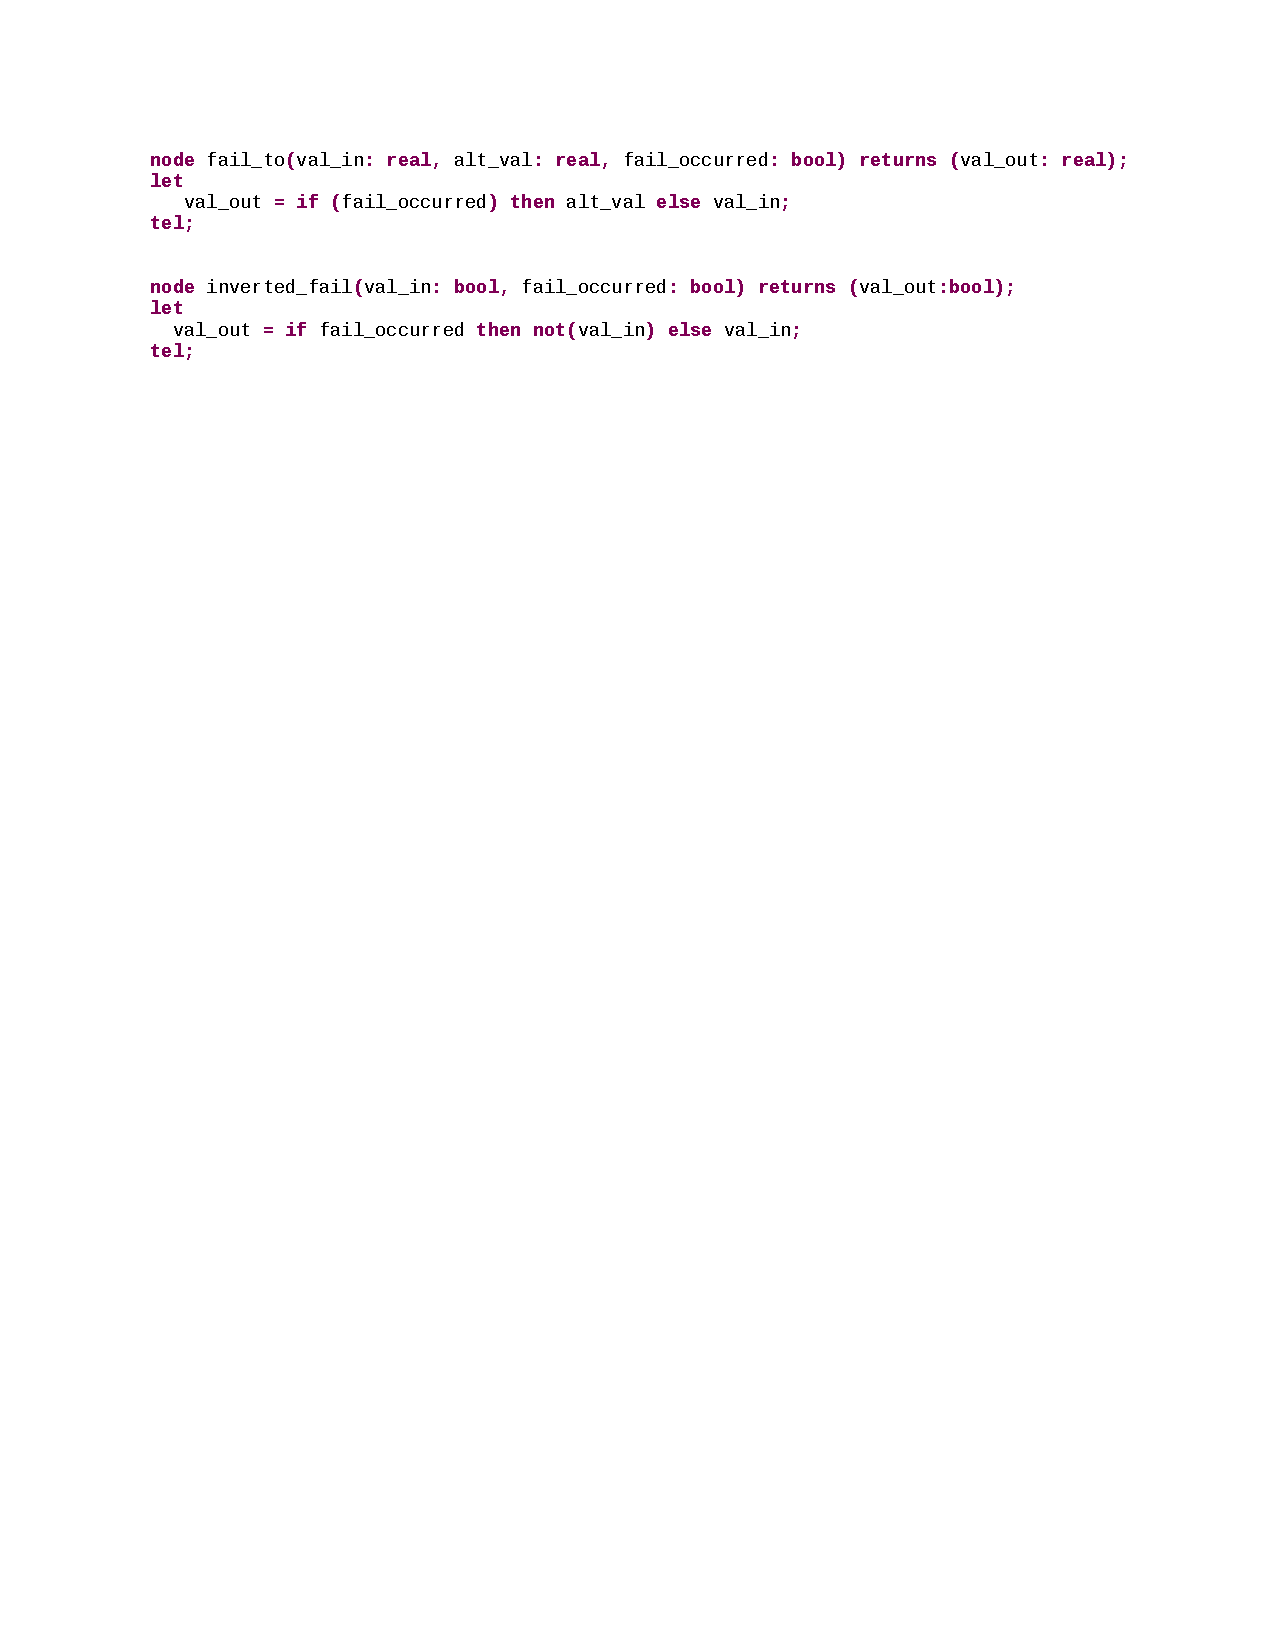
\includegraphics[trim=70 630 60 20,clip,width=1\textwidth]{images/fail_nodes.pdf}
  \vspace{-0.1in}
  \caption{AGREE Definition of a \textit{fail\_to} and \textit{inverted\_failure} Faults}
  \label{fig:failureNodes}
\end{figure}

These faults can be easily encoded in AGREE as shown in Figure~\ref{fig:failureNodes}.  The failures simply return an alternate value (for {\em fail\_to}) or invert the input value (for {\em inverted\_failure}) when a failure occurs.


While modeling faults, the duration of the fault must also be taken into account.  The AGREE tools allow a great deal of flexibility in terms of how faults are defined and their duration.  For the purposes of this model, we currently consider only {\em transient} and {\em permanent} faults, where transient faults occur for an instant in time (e.g., a single-event upset) and a permanent fault persists for the remainder of the system execution.


\subsection{Analysis of Faulty Models}
The following is a short summary of the failures defined in the fault model.

\begin{itemize}

\item Valves and Pumps: All valves and pumps have the possibility of a \textit{fail\_to} fault. This includes green pump, blue pump, accumulator, and the shutoff valves.

\item  The selector can also have a digital \textit{fail\_to} fault regarding the inputs from BSCU commanding to use normal or alternate means of pressure along with an \textit{inverted\_fail} fault which would change the boolean value that commands antiskid to activate.

\end{itemize}

Given our understanding of the WBS, our assumption was that any single permanent fault could be introduced into the system and the pilot would still be able to command brake pressure.  However, our analysis tools returned a counterexample to the property, and upon examination, the structure of the reference model was insufficient to guarantee the property.

%\subsection{Strengthening the Nominal Model}
The first issue was {\em feedback}; the reference model did not have a sensor to determine pressure after the selector valve.  This means that a single failure of (for example) the blue or green antiskid valve cannot be detected by the BSCU (see Figure~\ref{fig:wbs_ima}), and it cannot route around the failure.  In order to address this, we added a pressure sensor to the wheel that communicates with the BSCU to detect lack of pressure at the wheel.


After adding a sensing apparatus to the wheel, the analysis generated another counterexample due to a single failure of the selector valve.  In the reference model, there is a single selector component that takes as inputs the green pump, the blue pump, and the accumulator.  A single failure in this component can lead to no pressure along either of the two outgoing pressure lines.
To solve this issue, we removed the accumulator from the selector and added an accumulator valve.   This component takes in the blue pressure from the selector and the accumulator pressure. It also takes in a \textit{select\_alternate} flag from the BSCU. The output of the accumulator\_valve goes directly to the blue\_skid component and is either the blue or the accumulator pressure.

Finally, our BSCU is currently structured to always fail-over from the green system to the blue system but never the reverse.  Because of this choice (which matches the AIR6110 document), it is also necessary to guarantee that \textit{select\_alternate} is false until a failure occurs in the system; otherwise, a single failure in the blue anti-skid valve can cause the system to fail to provide pressure.  This asymmetry is something that could be revisited in future work.


Even after making these three changes to the model, the original property still does not prove.  At issue is that the sensing of a no-pressure situation is not instantaneous; there is a delay for this information to reach the BSCU and be acted upon to switch to the alternate braking system.  In our current timing model for the system, the feedback to the BSCU involves a delay, but the BSCU and valves can react.  Thus, we weaken our top-level property to state that if the brakes are pressed for two consecutive time instants, then pressure will be provided to the wheels:

\begin{tt}
\ \\
If pedals are pressed in the previous state and pressed in the current state and no skid occurs, then the brakes will receive pressure. \\
\end{tt}

The nominal WBS model extended with the faults described in this section can be found at \textit{https://github.com/loonwerks/AMASE}. 


















\section{Discussion}
We have used the WBS model as a vehicle to experiment with different modeling and fault representation ideas, and to get a feel for the scalability of our approach.
%
We started from the reference AADL model~\cite{SEI:AADL} to attempt to contrast our FEM approach using AGREE contracts vs. the FLM-based approach that was already part of this model.  Part of this was driven by curiosity as to whether important faults might be caught by one approach and missed by the other, and to contrast the two styles of analysis.

During the process of defining and injecting faults, subtle issues of the system structure and behavioral interactions became much clearer.  The idea that the system must use the green side until a failure occurs was unexpected.  In addition, the extensions to the model were driven by the counterexamples returned by the tools.   The approach quickly and precisely provided feedback towards aspects of the system that were not robust to failure.  The researcher who produced the model (Stewart) was not involved in earlier MBSA work and had no prior exposure to the WBS model and yet was able to relatively quickly construct a fault-tolerant model.  The fact that these holes in the reference model perhaps means that the behavioral approach can be better at drawing attention to certain kinds of failures.

On the other hand, the utility of the safety analysis is driven by the ``goodness'' of the properties.  Our one example property is clearly insufficient: for example, it is not possible to detect faults related to over-pressurization or misapplication of the brakes when no braking is commanded.  Of course, any complete analysis should have properties related to each hazardous condition.  The approach is foundationally a top-down analysis (like fault trees) rather than a bottom up approach (like a FMEA / FMECA).  In addition, if properties are mis-specified, or the system dynamics are incorrectly modeled, then properties may verify even when systems are unsafe.  The explicit propagation approach of the FLM techniques force the analyst to consider each fault interaction.  This too is a double-edged sword: when examining some of the fault propagations in the reference model, we disagreed with some of the choices made, particularly with respect to the selector valve.  For example, if no select alternate commands are received from the BSCU, then both the green and blue lines emit a {\em No\_Service} failure.

In terms of scalability, the analysis time for counterexamples was on the order of 1-2 seconds, and the time for proofs was around 4 seconds, even after annotating the model with several different failures.  From earlier experience applying compositional verification with the AGREE tools (e.g.,~\cite{QFCS15:backes,hilt2013}), we believe that the analysis will scale well to reasonably large models with many component failures, but this will be determined in future work.

The analysis in this paper involved hand-annotating the models with failure nodes.  This process is both schematic and straightforward: we define the AGREE contracts over internal {\em nominal output variables} and then define the actual outputs using the nominal output variables as inputs to the fault nodes like those in Figure~\ref{fig:failureNodes}.   We are currently in the process of defining a fault integration language which will eliminate the need for hand-annotation.  Some aspects of the Error Annex could be directly relevant: the state machines describing leaf-level faults could easily be compiled into behavioral state machines that determine when faults occur.  On the other hand, in a behavioral approach we need to be able to bring in additional quantities (inputs, parameters) to instantiate behavioral faults, and the two approaches have very different notions of propagation.

The xSAP tool~\cite{DBLP:conf/tacas/BittnerBCCGGMMZ16} has an elegant extension language that allows for fault definition, selection between multiple faults for a component, and ``global'' dependent faults that can affect multiple components.  The authors have used this support to construct a sophisticated analysis model for the WBS~\cite{DBLP:conf/cav/BozzanoCPJKPRT15}.  However, some useful aspects of fault modeling, such as global faults that are driven by the state of the model, appear to be hard to construct.  For example, a pipe-burst failure can be seen as a global failure because it may cause unconnected components within the model to fail, so can be represented as having a certain probability.  On the other hand, the likelihood of failure in the real system is driven by the number of currently pressurized pipes in the system, which appears to be hard to define.  We hope to allow for such conditional and model-driven failures in our fault definition language.





\section{Conclusion}

An extension to the AADL language has been developed with tool support for formal analysis of system safety properties in the presence of faults. Faulty behavior is specified as an extension of the nominal model, allowing safety analysis and system implementation to be driven from a single common model. This new Safety Annex leverages the AADL structural model and nominal behavioral specification (using the AGREE annex) to propagate faulty component behaviors without the need to add separate propagation specifications to the model.   Next steps will include extensions to automate injection of Byzantine faults as well as automatic generation of fault trees.  For more details on the tool, models, and approach, see the technical report and the repository~\cite{SATechReport, amaseRepo}.

\vspace{2 mm}
\noindent {\bf Acknowledgments.} This research was funded by NASA contract NNL16AB07T and the University of Minnesota College of Science and Engineering Graduate Fellowship.



%ACKNOWLEDGMENTS are optional
%TODO: Fill in for final version
\vspace{0.08in}


%\textbf{Acknowledgments:}
%This work was supported by

%We thank XXXX

\bibliographystyle{abbrv}
\bibliography{biblio}

% This ~ seems to fix an odd bibliography alignment issue
~

%\ifdefined\TECHREPORT
%\appendix
%
%\section{Appendix: Proof of Equivalence}
%\input{appendix}
%\fi

%\section{Appendix: GPCA CENTA Model}
%\label{appendix:gpcacenta}
%\begin{figure}[!ht]
%\begin{center}
%\includegraphics[scale=0.6]{images/sampled_pca.PNG} %[trim = 0 2 0 0, clip=true]{Comp}
%\caption{GPCA AGREE Properties modeled as a Timed Automata} \label{fig:samplepca}
%\end{center}
%\end{figure}

%\balancecolumns

\end{document}
